\documentclass[tikz]{standalone}
\usetikzlibrary{calc}

\definecolor{blue}{HTML}{1F78B4}
\definecolor{red}{HTML}{E31A1C}
\definecolor{grey80}{HTML}{CCCCCC}

\begin{document}
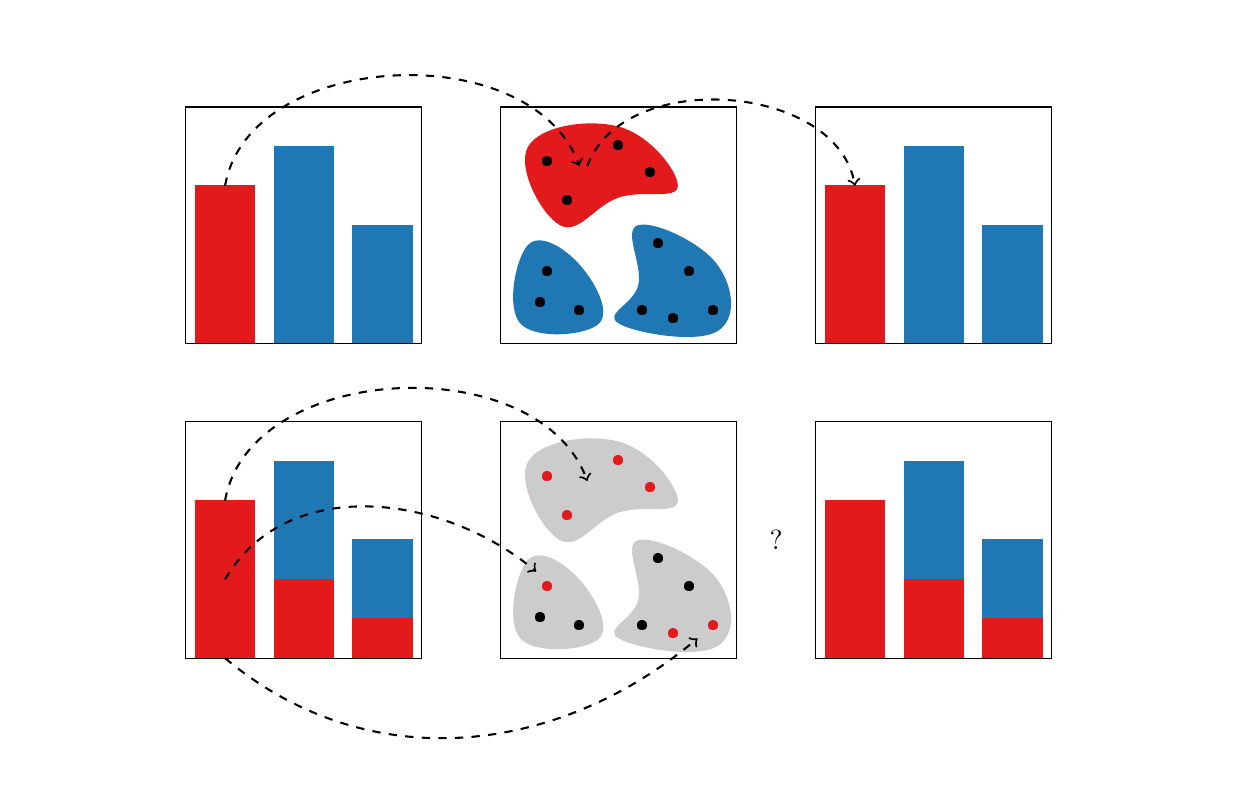
\begin{tikzpicture}[scale=1.0]

  \filldraw[white] (-2, -1) rectangle (13, 8);

  % START OF THE TOP ROW

  % BARS LEFT
  \filldraw[red] (0.125, 4) rectangle ++(0.75, 2);
  \filldraw[blue] (1.125, 4) rectangle ++(0.75, 2.5);
  \filldraw[blue] (2.125, 4) rectangle ++(0.75, 1.5);

  % BARS RIGHT
  \filldraw[red] (8.125, 4) rectangle ++(0.75, 2);
  \filldraw[blue] (9.125, 4) rectangle ++(0.75, 2.5);
  \filldraw[blue] (10.125, 4) rectangle ++(0.75, 1.5);

  % SETS
  \fill[blue] plot [smooth cycle, tension=0.75] coordinates {
    (4.25, 4.25) (4.35, 5.25) (5, 5) (5.25, 4.25) } -- cycle;
  \foreach \point in {(4.5,4.5), (4.6, 4.9), (5, 4.4)}{
    \node at \point {\textbullet};
  }

  \fill[red] plot [smooth cycle, tension=0.75] coordinates {
    (4.35, 6.5) (5.5, 6.75) (6.25, 6) (5.5, 5.85) (4.75, 5.5) } -- cycle;
  \foreach \point in {(4.6, 6.3), (5.5, 6.5), (5.9, 6.15), (4.85, 5.8)}{
    \node at \point {\textbullet};
  }

  \fill[blue] plot [smooth cycle, tension=0.75] coordinates {
    (5.5, 4.25) (6.75, 4.15) (6.75, 5) (5.75, 5.5) (5.75, 4.75) } -- cycle;
  \foreach \point in {(5.8, 4.4), (6.2, 4.3), (6.7, 4.4), (6.4, 4.9), (6, 5.25)}{
    \node at \point {\textbullet};
  }

  % ARROWS
  \draw[->,line width=0.75,dashed] (0.5, 6) to[out=80, in=110] (5, 6.25);
  \draw[->,line width=0.75,dashed] (5.1, 6.25) to[out=70, in=100] (8.5, 6);

  % BOXES
  \draw[black] (0, 4) rectangle ++(3, 3);
  \draw[black] (4, 4) rectangle ++(3, 3);
  \draw[black] (8, 4) rectangle ++(3, 3);

  %%%%

  % START OF THE BOTTOM ROW

    % BARS LEFT
  \filldraw[red] (0.125, 0) rectangle ++(0.75, 2);
  \filldraw[blue] (1.125, 0) rectangle ++(0.75, 2.5);
  \filldraw[red] (1.125, 0) rectangle ++(0.75, 1);
  \filldraw[blue] (2.125, 0) rectangle ++(0.75, 1.5);
  \filldraw[red] (2.125, 0) rectangle ++(0.75, 0.5);

  % BARS RIGHT
  \filldraw[red] (8.125, 0) rectangle ++(0.75, 2);
  \filldraw[blue] (9.125, 0) rectangle ++(0.75, 2.5);
  \filldraw[red] (9.125, 0) rectangle ++(0.75, 1);
  \filldraw[blue] (10.125, 0) rectangle ++(0.75, 1.5);
  \filldraw[red] (10.125, 0) rectangle ++(0.75, 0.5);

  % SETS
  \fill[grey80] plot [smooth cycle, tension=0.75] coordinates {
    (4.25, 0.25) (4.35, 1.25) (5, 1) (5.25, 0.25) } -- cycle;
  \foreach \point in {(4.5,0.5), (5, 0.4)}{
    \node at \point {\textbullet};
  }
  \node [red] at (4.6, 0.9) {\textbullet};

  \fill[grey80] plot [smooth cycle, tension=0.75] coordinates {
    (4.35, 2.5) (5.5, 2.75) (6.25, 2) (5.5, 1.85) (4.75, 1.5) } -- cycle;
  \foreach \point in {(4.6, 2.3), (5.5, 2.5), (5.9, 2.15), (4.85, 1.8)}{
    \node [red] at \point {\textbullet};
  }

  \fill[grey80] plot [smooth cycle, tension=0.75] coordinates {
    (5.5, 0.25) (6.75, 0.15) (6.75, 1) (5.75, 1.5) (5.75, 0.75) } -- cycle;
  \foreach \point in {(5.8, 0.4), (6.4, 0.9), (6, 1.25)}{
    \node at \point {\textbullet};
  }
  \node [red] at (6.2, 0.3) {\textbullet};
  \node [red] at (6.7, 0.4) {\textbullet};


  % ARROWS
  \draw[->,line width=0.75,dashed] (0.5, 2) to[out=80, in=110] (5.1, 2.25);
  \draw[->,line width=0.75,dashed] (0.5, 0) to[out=320, in=220] (6.5, 0.25);
  \draw[->,line width=0.75,dashed] (0.5, 1) to[out=60, in=140] (4.45, 1.1);


  % BOXES
  \draw[black] (0, 0) rectangle ++(3, 3);
  \draw[black] (4, 0) rectangle ++(3, 3);
  \draw[black] (8, 0) rectangle ++(3, 3);

  \node at (7.5, 1.5) {?};

\end{tikzpicture}
\end{document}
